\chapter{Related Works}

Your related works, and your purpose and contribution which must be different as below.


\section{puad hamdani/1164084}
\subsection{binary classification }
\begin{enumerate}
\item Output aktual dari banyak algoritma binary classification adalah skor prediksi. Skor menunjukkan kepastian sistem bahwa pengamatan yang diberikan adalah milik kelas positif. Untuk membuat keputusan tentang apakah pengamatan harus diklasifikasikan sebagai positif atau negatif
\end{enumerate}

\subsection{supervised learning dan unsupervised learning}
\begin{enumerate}
\item Supervised learning adalah sebuah pendekatan dimana sudah terdapat data yang dilatih, dan terdapat variable yang di targetkan sehingga tujuan dari pendekatan ini adalah mengelompokkan suatu data ke data yang sudah ada.


\item Unsupervised learning adalah istilah yang digunakan untuk pembelajaran bahasa Ibrani, yang terkait dengan pembelajaran tanpa guru, juga dikenal sebagai organisasi mandiri dan metode pemodelan kepadatan probabilitas input. Unsupervised learning tidak memiliki data latih, sehingga dari data yang ada, kita mengelompokan data tersebut menjadi dua bagian atau tiga bagian dan seterusnya.
\end{enumerate}

\subsection{evaluasi dan akurasi }
\begin{enumerate}
\item Evaluasi merupakan suatu proses identifikasi untuk mengukur atau menilai apakah suatu kegiatan/program yang dilaksanakan sesuai dengan perencanaan atau tujuan yang ingin dicapai.
Akurasi merupakan tingkat kedekatan pengukuran kuantitas terhadap nilai yang sebenarnya. Kepresisian dari suatu sistem pengukuran
\end{enumerate}

\subsection{ bagaimana cara membuat dan membaca confusion matrix, buat confusion matrix }
\begin{enumerate}
\item Cara membuat dan membaca confusion matrix :
\begin{itemize}
\item 1)	Tentukan pokok permasalahan dan atributanya
\item 2)	Buat pohon keputusan
\item 3)	Lalu data testingnya
\item 4)	Lalu mencari nilai a, b, c, dan d. Semisal a = 5, b = 1, c = 1, dan d = 3.
\item 5)	Selanjutnya mencari nilai recall, precision, accuracy, serta dan error rate.
\end{itemize}
\item Berikut adalah contoh dari confusion matrix :
\begin{itemize}
\item Recall =3/(1+3) = 0,75
\item Precision = 3/(1+3) = 0,75
\item Accuracy =(5+3)/(5+1+1+3) = 0,8
\item Error Rate =(1+1)/(5+1+1+3) = 0,2
\end{itemize}
\end{enumerate}

\subsection{bagaimana K-fold cross validation bekerja dengan gambar ilustrasi}
\begin{enumerate}
\item Cara kerja K-fold cross validation :
\begin{itemize}
\item 1)	Total instance dibagi menjadi N bagian.
\item 2)	Fold yang pertama adalah bagian pertama menjadi data uji (testing data) dan sisanya menjadi training data.
\item 3)	Lalu hitung akurasi berdasarkan porsi data tersebut dengan menggunakan persamaan.
\item 4)	Fold yang ke dua adalah bagian ke dua menjadi data uji (testing data) dan sisanya training data. 
\item 5)	Kemudian hitung akurasi berdasarkan porsi data tersebut.
\item 6)	Dan seterusnya hingga habis mencapai fold ke-K.
\item 7)	Terakhir hitung rata-rata akurasi K buah.
\end{itemize}
\end{enumerate}

\subsection{decision tree}
\begin{enumerate}
\item Decision tree merupakan model prediksi menggunakan struktur pohon atau struktur berhirarki.
\end{enumerate}

\subsection{Information Gain}
\begin{enumerate}
\item Information gain. Metode tersebut akan melakukan proses komputasi untuk mendapatkan atribut-atribut yang paling berpengaruh terhadap dataset
\end{enumerate}


\section{Puad Hamdani/ 1164084}
\subsection{Scikit-Learn}

\begin{enumerate}
\item
\begin{verbatim}
	# load dataset (student mat pakenya)
	import pandas as pd
	sate    = pd.read_csv('student-mat.csv', sep=';')
	len(sate)
\end{verbatim}
\begin{figure}[ht]
\centering
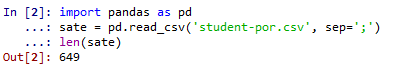
\includegraphics[scale=0.5]{figures/41.png}
\caption{Load Dataset}
\end{figure}
\par
	Codingan ini akan meload ( menampilkan ) data pada file yang ditentukan. hasilnya berupa angka 649 . 

\item
\begin{verbatim}
	# generate binary label (pass/fail) based on G1+G2+G3 
	# (test grades, each 0-20 pts); threshold for passing is sum>=30
	sate['pass'] = sate.apply(lambda row: 1 if (row['G1']+row['G2']+row['G3']) 
											>= 35 else 0, axis=1)
	sate = sate.drop(['G1', 'G2', 'G3'], axis=1)
	sate.head()
\end{verbatim}
\begin{figure}[ht]
\centering
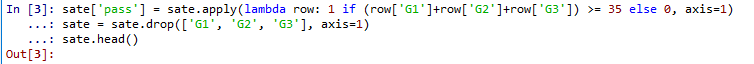
\includegraphics[scale=0.6]{figures/42.png}
\caption{Generate Binary Label}
\end{figure}
\par
	Codingan ini secara keseluruhan menampilkan  baris  G1, G2 dan G3 ( berdasarkan kriterianya ). Untuk lebih jelasnya, pada codingan terdapat pendefinisian pembacaan "lambda" ( panjang gelombang ) dari baris G1, G2 dan G3. Apabila row-row tersebut bernilai lebih dari 35 maka akan terdefinisikan angka "1" apabila tidak, maka akan terdefinisikan angka "0"
\item
\begin{verbatim}
	# use one-hot encoding on categorical columns
	sate = pd.get_dummies(sate, columns=['sex', 'school', 'address', 
									'famsize', 
									'Pstatus', 'Mjob', 'Fjob', 
	                               'reason', 'guardian', 'schoolsup', 
								   'famsup', 'paid', 'activities',
	                               'nursery', 'higher', 'internet', 
									'romantic'])
	sate.head()
\end{verbatim}
\begin{figure}[ht]
\centering
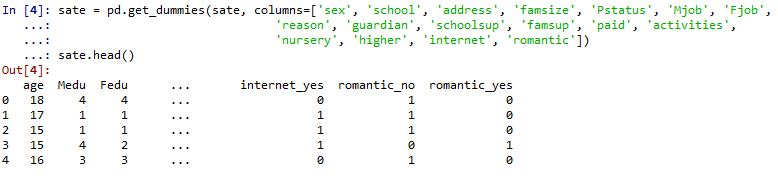
\includegraphics[scale=0.6]{figures/421.png}
\caption{Pemanggilan get dummies}
\end{figure}
\par
	Secara keseluruhan, codingan ini mendefinisikan pemanggilan get dummies ke dalam variabel sate.

\item
\begin{verbatim}
	# shuffle rows
	sate = sate.sample(frac=1)
	# split training and testing data
	sate_train = d[:500]
	sate_test = d[500:]

	sate_train_att = sate_train.drop(['pass'], axis=1)
	sate_train_pass = sate_train['pass']

	sate_test_att = sate_test.drop(['pass'], axis=1)
	sate_test_pass = sate_test['pass']

	sate_att = sate.drop(['pass'], axis=1)
	sate_pass = sate['pass']

	# number of passing students in whole dataset:
	import numpy as np
	print("Passing: %d out of %d (%.2f%%)" % (np.sum(lontong_pass), len(lontong_pass), 
	       100*float(np.sum(sate_pass)) / len(sate_pass)))
\end{verbatim}
\begin{figure}[ht]
\centering
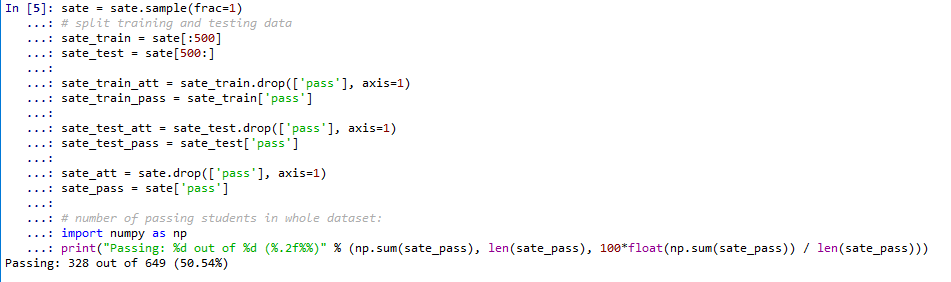
\includegraphics[scale=0.6]{figures/43.png}
\caption{Mendefinisikan pembagian data}
\end{figure}
\par
	Secara keseluruhan codingan ini difungsikan untuk mendefinisikan pembagian data yang berupa training dan testing data

\item 
\begin{verbatim}
	# fit a decision tree
	from sklearn import tree
	rendang = tree.DecisionTreeClassifier(criterion="entropy", max_depth=5)
	rendang = rendang.fit(sate_train_att, sate_train_pass)
\end{verbatim}
\begin{figure}[ht]
\centering
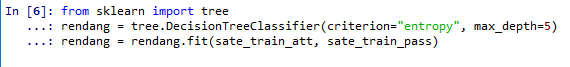
\includegraphics[scale=0.9]{figures/44.png}
\caption{Membuktikan pengujian}
\end{figure}
\par
	Secara keseluruhan, codingan ini hanya membuktikan pengujian dari Klasifikasi Decision Tree yang ada, apakah true atau tidak dan hasilnya true

\item
\begin{verbatim}
	# visualize tree
	import graphviz
	dot_data = tree.export_graphviz(rendang, out_file=None, label="all", 
									impurity=False, proportion=True,
	                                feature_names=list(sate_train_att), 
									class_names=["fail", "pass"], 
	                                filled=True, rounded=True)
	graph = graphviz.Source(dot_data)
	graph
\end{verbatim}
\begin{figure}[ht]
\centering
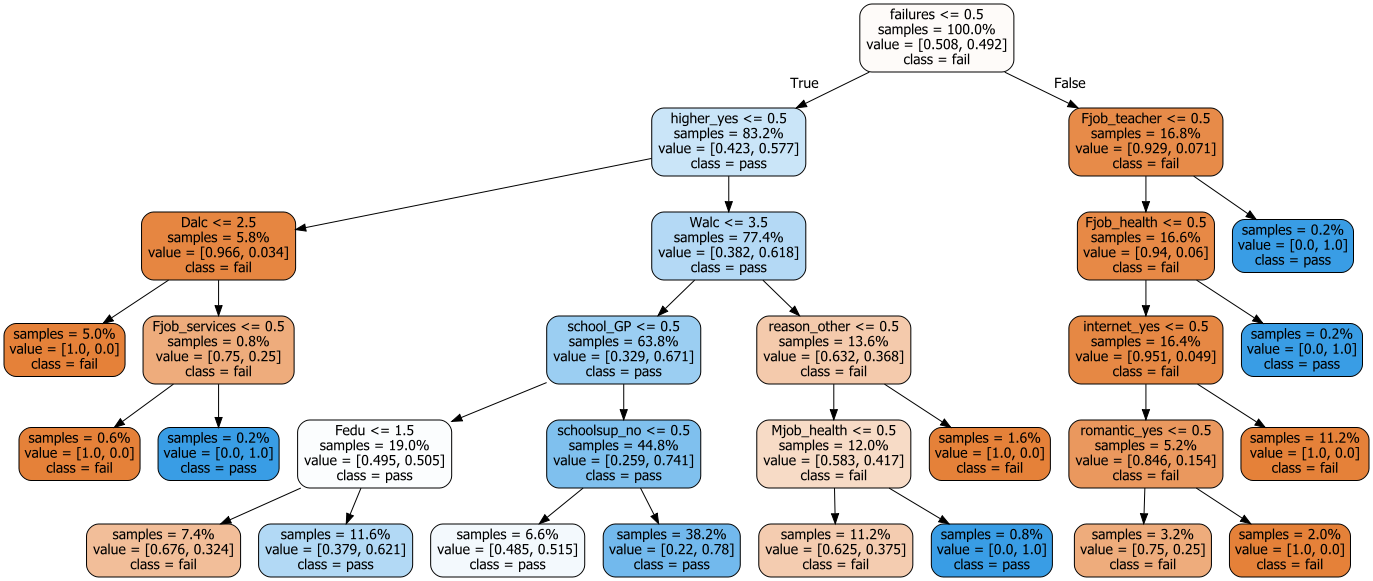
\includegraphics[scale=0.3]{figures/45.png}
\caption{Gambaran decision tree}
\end{figure}
\par
	Codingan ini memberikan gambaran dari klasifikasi decision tree dari pengolahan parameter yang dieksekusi kedalam variabel soto. Tentunya dengan pemanfaatan library graphviz yang telah diimport dan difungsikan.

\item
\begin{verbatim}
	# save tree
	tree.export_graphviz(rendang, out_file="student-performance.dot", 
						 label="all", impurity=False, 
						 proportion=True,
	                     feature_names=list(sate_train_att), 
	                     class_names=["fail", "pass"], 
	                     filled=True, rounded=True)
\end{verbatim}
\begin{figure}[ht]
\centering
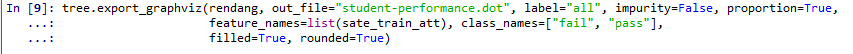
\includegraphics[scale=0.6]{figures/46.png}
\caption{Library Graphviz}
\end{figure}
\par
	Pada gambar 4.6 akan menampilkan yang terdapat pada Library Graphviz,
\item
\begin{verbatim}
	rendang.score(sate_test_att, sate_test_pass)
\end{verbatim}
\begin{figure}[ht]
\centering
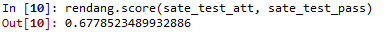
\includegraphics[scale=0.9]{figures/47.png}
\caption{Menampilkan hasil perhitungan 2 parameter}
\end{figure}
\par
	merupakan perhitungan hasil prediksi silang akan kemungkinan nilai di masa mendatang.

\item
\begin{verbatim}
	from sklearn.model_selection import cross_val_score
	semur = cross_val_score(rendang, sate_att, sate_pass, cv=5)
	# show average score and +/- two standard deviations away 
	#(covering 95% of scores)
	print("Accuracy: %0.2f (+/- %0.2f)" % (semur.mean(), semur.std() * 2))
\end{verbatim}
\begin{figure}[ht]
\centering
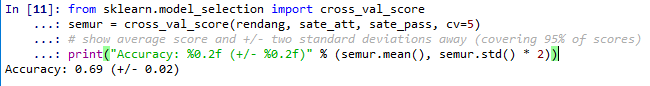
\includegraphics[scale=0.6]{figures/48.png}
\caption{Mendefinisikan library sklearn}
\end{figure}
\par
	Kodingan tersebut mendefinisikan library sklearn model selection dan import cross val score
\item 
\begin{verbatim}
	for max_depth in range(1, 20):
	    rendang = tree.DecisionTreeClassifier(criterion="entropy", 
			max_depth=max_depth)
	    semur = cross_val_score(rendang, sate_att, sate_pass, cv=5)
	    print("Max depth: %d, Accuracy: %0.2f (+/- %0.2f)" % 
				(max_depth, semur.mean(), semur.std() * 2)
			 )
\end{verbatim}
\begin{figure}[ht]
\centering
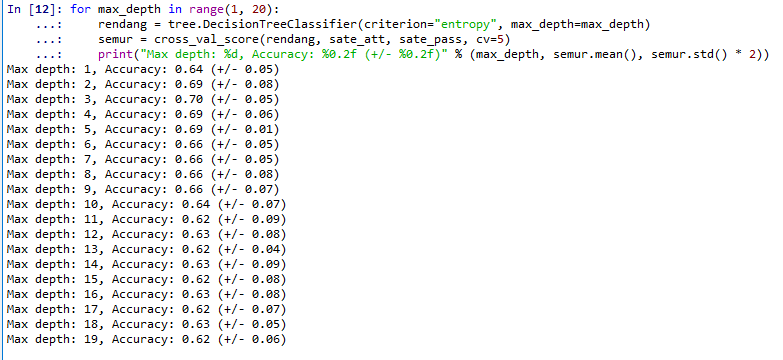
\includegraphics[scale=0.6]{figures/49.png}
\caption{Menampilkan hasil fungsi max depth dan accuracy}
\end{figure}
\par
	menmpilkan data dari angka 1-20.

\item
\begin{verbatim}
	depth_acc = np.empty((19,3), float)
	i = 0
	for max_depth in range(1, 20):
	    soto = tree.DecisionTreeClassifier(criterion="entropy", 
			max_depth=max_depth)
	    semur = cross_val_score(rendang, sate_att, sate_pass, cv=5)
	    depth_acc[i,0] = max_depth
	    depth_acc[i,1] = semur.mean()
	    depth_acc[i,2] = semur.std() * 2
	    i += 1

	depth_acc
\end{verbatim}
\begin{figure}[ht]
\centering
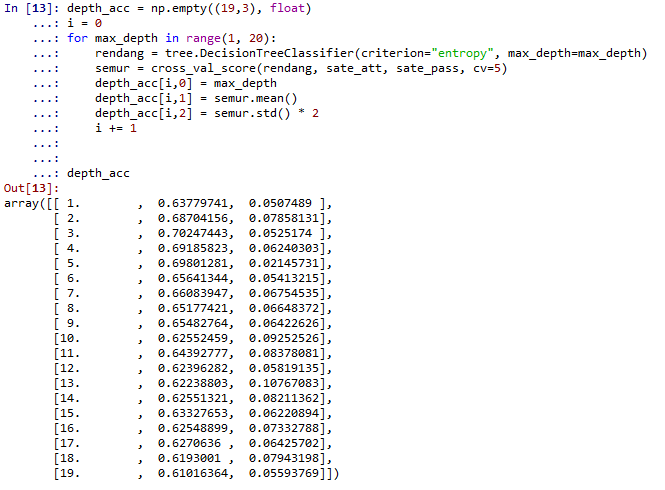
\includegraphics[scale=0.6]{figures/410.png}
\caption{Menjelaskan variable kari}
\end{figure}
\par
	Bahwa variable semur akan menampilkan atau mendefinisikan nilai dari variabel score yang mana isi dari variable score yaitu rendang

\item 
\begin{verbatim}
	import matplotlib.pyplot as plt
	fig, ax = plt.subplots()
	ax.errorbar(depth_acc[:,0], depth_acc[:,1], yerr=depth_acc[:,2])
	plt.show()
\end{verbatim}
\begin{figure}[ht]
\centering
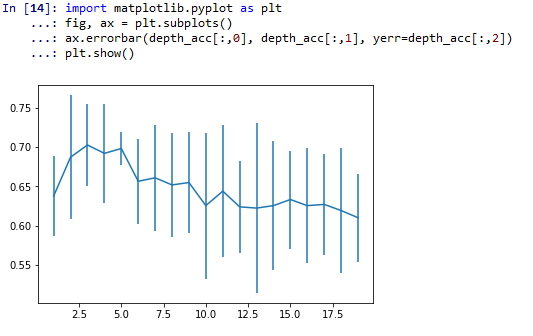
\includegraphics[scale=0.5]{figures/411.png}
\caption{Menjelaskan dan menampilkan gambar grafik}
\end{figure}
\par
	menampilkan gambar grafik pada gambar 4.11 dari eksekusi fungsi ax.errorbar.

\end{enumerate}


\section{Penanganan Error}
Dari percobaan yang dilakukan di atas, tidak ada eror:


\section{Same Topics}
Cite every latest journal with same topic
\subsection{Topic 1}
cite for first topic

\subsection{Topic 2}
if you have two topics you can include here to


\section{Same Method}
write and cite latest journal with same method

\subsection{Method 1}
cite and paraphrase method 1

\subsection{Method 2}
cite and paraphrase method 2 if you have more method please add new subsection.

 

